\documentclass[a4paper]{article}
\usepackage{array}
\usepackage{algorithmicx}
\usepackage{algpseudocode}
\usepackage{amssymb}
\usepackage{tabu}
\usepackage{longtable}
\usepackage[table]{xcolor}
\usepackage{hyperref}
\usepackage{float}
\usepackage{wrapfig}
\usepackage[utf8]{inputenc}
\usepackage{graphicx}
\usepackage{pgfgantt}
\usepackage{amsmath}
\usepackage{tikz}
\usepackage[margin=1 in]{geometry}
\usepackage{color}
\usepackage{caption}
\usepackage{subcaption}
\usepackage[usenames,dvipsnames]{pstricks}
\usepackage{epsfig}
\usepackage{textcomp}
\definecolor{listinggray}{gray}{0.9}
\usepackage{listings}
\lstset{
	language=,
	literate=
		{æ}{{\ae}}1
		{ø}{{\o}}1
		{å}{{\aa}}1
		{Æ}{{\AE}}1
		{Ø}{{\O}}1
		{Å}{{\AA}}1,
	backgroundcolor=\color{listinggray},
	tabsize=3,
	rulecolor=,
	basicstyle=\scriptsize,
	upquote=true,
	aboveskip={0.2\baselineskip},
	columns=fixed,
	showstringspaces=false,
	extendedchars=true,
	breaklines=true,
	prebreak =\raisebox{0ex}[0ex][0ex]{\ensuremath{\hookleftarrow}},
	frame=single,
	showtabs=false,
	showspaces=false,
	showlines=true,
	showstringspaces=false,
	identifierstyle=\ttfamily,
	keywordstyle=\color[rgb]{0,0,1},
	commentstyle=\color[rgb]{0.133,0.545,0.133},
	stringstyle=\color[rgb]{0.627,0.126,0.941},
  moredelim=**[is][\color{blue}]{@}{@},
}

\lstdefinestyle{base}{
  emptylines=1,
  breaklines=true,
  basicstyle=\ttfamily\color{black},
}

\definecolor{barblue}{RGB}{153,204,254}
\definecolor{groupblue}{RGB}{51,102,254}
\definecolor{linkred}{RGB}{165,0,33}
\def\sfm*{\texttt{scan\_for\_matches}}
\def\E{\mathbb{E}}
\def\V{\mathbb{V}ar}
\def\P{\mathbb{P}}
\def\H{\mathcal{H}}
\def\qvec#1#2{\begin{bmatrix} #1 \\ #2 \end{bmatrix}}
\makeatletter
\renewcommand{\ALG@beginalgorithmic}{\footnotesize}
\makeatother
\usetikzlibrary{shapes}
\title{Machine Learning\\Assignment 1.1 - Classification and Concentration Bounds}
\author{Tobias Hallundbæk Petersen - xtv657}
\begin{document}
\maketitle
\section{Classification}
\subsection{Nearest neighbor}
I have used NumPy for this implementation as it greatly improves performance and generally makes your code neater and more readable. The following is my source code for my nearest neighbor classifier:
\lstinputlisting[language=Python, firstline=15, lastline=19]{./ass1.py}
The implementation is very general and allows any given distance metric to be used, this function given to compute the distance, should be able to return a list of distances given the training set data and a target. For the next line, we find the indices of the $k$ shortest distances, the next line counts the different classifications and then returns the maximum of these.
If the program is run with the parameter \texttt{1.1} we get the following output:
\begin{lstlisting}
Error of the 1-nn classifier: 0.184210526316
Error of the 3-nn classifier: 0.184210526316
Error of the 5-nn classifier: 0.315789473684
\end{lstlisting}
We can see both the 1-nn and 3-nn perform equally well, while the 5-nn has a quite much larger error, due to the small size of our training set this makes sense.
\subsection{Hyperparameter selection using cross-validation}
For the cross validation I have partitioned the training set into 5 sets, and run $k$-nn for $k$ from $\{1,3,5,...,25\}$ for the five tests, these tests and their division can be seen in Figure \ref{12}.
\begin{figure}[H]
  \centering
  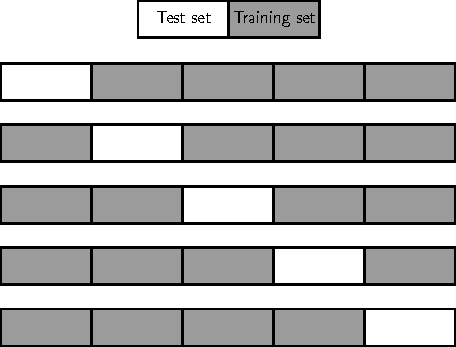
\includegraphics[width=0.7\textwidth]{./12.pdf}
  \caption{Division of the training set for use in cross-validation}
  \label{12}
\end{figure}
For this I implemented the more general $n$-fold cross-validation. This was implemented in the following way.
\lstinputlisting[language=Python, firstline=37, lastline=51]{./ass1.py}
The data is split and then the cross validation is performed, it returns the average error over the $n$ different runs.\\
To get the results for $k$ from $\{1,3,5,...,25\}$ the program can be run with the \texttt{1.2} parameter, which yields the following response:
\begin{lstlisting}
Crossvalidation error for the k-nn classifier for k=[1,3 ... 25]
1-nn: 0.22
3-nn: 0.21
5-nn: 0.25
7-nn: 0.23
9-nn: 0.22
11-nn: 0.22
13-nn: 0.22
15-nn: 0.21
17-nn: 0.21
19-nn: 0.22
21-nn: 0.21
23-nn: 0.22
25-nn: 0.21

Best k found was 3 with an error of 0.21
\end{lstlisting}
And we see that the program suggests setting $k=3$, ties are in my program won by the first to get the best error.
\subsection{Data Normalization}
We want to normalize our training data and get a function $f_{norm}$ that when applied on the training data will conform the training data to have a 0 mean, 1 variance features. This function will then be used on the test set as well, this will not ensure that the test set will conform to the same restrictions as our training set but it should, given a large enough sample be close. \\
To normalize the data, the mean of the data is subtracted from the data, and the data is afterwards divided by its standard deviation, this will ensure that we get 0 mean, 1 variance features.\\
To get the results required in the assignment, the program can be run the \texttt{1.3} parameter, giving the following response:
\begin{lstlisting}
Original training data:
First feature, mean: 5.756, variance: 0.688864
Second feature, mean: 0.3017, variance: 0.00174211

Normalized test data:
First feature, mean: 0.208375768039, variance: 1.07339795338
Second feature, mean: 0.432138257729, variance: 1.25222270424

Crossvalidation error for the k-nn classifier for k=[1,3 ... 25] on normalized test data
1-nn: 0.14
3-nn: 0.18
5-nn: 0.18
7-nn: 0.19
9-nn: 0.16
11-nn: 0.14
13-nn: 0.15
15-nn: 0.2
17-nn: 0.19
19-nn: 0.16
21-nn: 0.16
23-nn: 0.16
25-nn: 0.16

Best k found was 1 with an error of 0.14
Error of the 1-nn classifier on normalized data: 0.214736842105
\end{lstlisting}
We can see that the normalization of the test data is not strictly 0 mean, 1 variance, but its a good way there. It is a bit disappointing that the error after all this normalization is worse than the one before normalization, but I would suppose that given a larger sample the normalization could improve upon the $k$-nn algorithm.
\section{Probability theory refreshment}
We have an urn that contains five red, three orange, and one blue ball. We now select two balls at random
\begin{enumerate}
  \item \textbf{What is the sample space of this experiment}\\
    $\{\{R,R\},\{R,O\},\{R,B\},\{O,O\},\{O,R\},\{O,B\},\{B,R\},\{B,O\}\}$
  \item \textbf{What is the probability of each point in the sample space}\\
    If we use the same ordering as above, $\{5/18,5/24,5/72,1/12,5/24,1/24,5/72,1/24\}$, the sum of these probabilities sum up to one, meaning that we have a complete sample space.
  \item \textbf{Let $X$ represent the number of orange balls selected. What are the possible values of $X$?}\\
    The possible values of $X$ are $\{0,1,2\}.$
  \item \textbf{Calculate $\P\{X=0\}$}\\
    $5/18 + 5/72 + 5/72 = 5/12$
  \item \textbf{Calculate $\E[X]$}\\
    $5/24 + 1/12 \cdot 2 + 5/24 + 1/24 + 1/24 = 2/3$
\end{enumerate}
\section{Probability theory refreshment}
From probability theory we have the following definitions and properties:
\begin{align*}
(a) &\ p_X(x)=\sum_{y\in \mathcal{Y}}p_{XY}(x,y) \\
(b) &\ \mbox{If $X$ and $Y$ are independent, then $P_{XY}(x,y)=p_X(x)p_Y(y)$} \\
(c) &\ \mathbb{E}[X]=\sum_{x\in \mathcal{X}}xp_X(x)
\end{align*}
$X$ and $Y$ are discrete random variables that take values from in $\mathcal{X}$ and $\mathcal{Y}$. $p_X$ is the distribution of $X$, $p_Y$ the distribution of $Y$ and $p_{XY}$ the distribution of $X$ and $Y$.

\subsection*{1.}
We prove the following identity:
\begin{align*}
\mathbb{E}[X+Y]=\mathbb{E}[X]+\mathbb{E}[Y]
\end{align*}
By (c), the expected value of $X$ is given by:
$$\mathbb{E}[X]=\sum_{x\in \mathcal{X}}xp_X(x)$$
Therefore the expected value of $X+Y$ would be
\begin{align*}
\mathbb{E}[X+Y] &=\sum_{x\in \mathcal{X}}\sum_{y\in \mathcal{Y}} (x+y)p_{XY}(x,y) \\
                &= \sum_{x\in \mathcal{X}}x\sum_{y\in \mathcal{Y}} p_{XY}(x,y)+ \sum_{y\in \mathcal{Y}}y\sum_{\in \mathcal{X}} p_{XY}(x,y) \\
                &= \sum_{x\in \mathcal{X}}xp(x)+\sum_{y\in \mathcal{Y}}yp(y) \\
                &= \mathbb{E}[X]+\mathbb{E}[Y]
\end{align*}
In the last step we use the definition for the expected value of a random variable. We have now shown that $\mathbb{E}[X+Y]=\mathbb{E}[X]+\mathbb{E}[Y]$.
\subsection*{2.}
To prove the following identity, we use that the random variables $X$ and $Y$ are independent.
\begin{align*}
\mathbb{E}[XY]=\mathbb{E}[X]\mathbb{E}[Y]
\end{align*}
We can write $\mathbb{E}[XY]$ as
\begin{align*}
\mathbb{E}[XY]           &= \sum_{x\in \mathcal{X}}\sum_{y\in \mathcal{Y}} xy p_{XY}(x,y)\\
\end{align*}
This is where we use that $X$ and $Y$ are independent - using property (b):
\begin{align*}
\sum_{x\in \mathcal{X}}\sum_{y\in \mathcal{Y}} xyp_{X}(x)p_{Y}(y)
\end{align*}
This can be reduced to prove our identity
\begin{align*}
\sum_{x\in \mathcal{X}}\sum_{y\in \mathcal{Y}} xyp_{X}(x)p_{Y}(y) &= \sum_{x\in \mathcal{X}}xp_{X}(x)\sum_{y\in \mathcal{Y}} yp_{Y}(y) \\
&= \mathbb{E}[X]\mathbb{E}[Y]
\end{align*}
This proves the identity $\mathbb{E}[XY]=\mathbb{E}[X]\mathbb{E}[Y]$.

\subsection*{3.}
A bag has $2$ red apples and $2$ green apples. There is taken $2$ apples from the bag without putting them back into the bag. Let $X$ be the first apple and let $Y$ be the second apple. The joint distribution table of $X$ and $Y$ is seen below:
\begin{center}
\begin{tabular}{|c||c|c|}
\hline
X / Y & Red & Green \\
\hline
\hline
Red & $\frac{1}{6}$  & $\frac{2}{6}$ \\
\hline
Green & $\frac{2}{6}$ & $\frac{1}{6}$\\
\hline
\end{tabular}
\end{center}
The probability of apple $X$ being red is:
\begin{align*}
\mathbb{E}[X=\mbox{Red}] = \frac{1}{2}
\end{align*}
Which is the same probability for apple $Y$ being red. We have that
\begin{align*}
\mathbb{E}[X=\mbox{Red} \land Y=\mbox{Red}]=\frac{1}{6}
\end{align*}
Since $\frac{1}{2}\frac{1}{2} = \frac{1}{4}\neq\frac{1}{6}$ then
\begin{align*}
\mathbb{E}[XY]\neq \mathbb{E}[X]\mathbb{E}[Y]
\end{align*}
in this example.

\subsection*{4.}
The identity to be proved:
\begin{align*}
\mathbb{E}[\mathbb{E}[X]]=\mathbb{E}[X]
\end{align*}
We know that $\mathbb{E}[X]=k$ and that $\mathbb{E}[k]=k$. That means taking the expected value of an expected value will just return the constant you already found. This can be done more than $2$ times and it will always be the constant $k$ that is your result.

\subsection*{5.}
We want to show that $\E[(X-\E[X])^2] = \E[X^2]-(\E[X])^2.$
\begin{align*}
  \E[(X-\E[X])^2] &= \E[X^2 - 2\cdot X \cdot \E[X]+ (\E[X])^2]\\
                  &= \E[X^2] - 2\cdot \E[X] \cdot \E[X] + (\E[X])^2\\
                  &= \E[X^2]-(\E[X])^2
\end{align*}
\section{Markov's inequality vs. Hoeffding's inequality vs. binomial bound}
We let $X_1,...,X_{10}$ be i.i.d. Bernolli random variables with bias $1/2$.
\begin{enumerate}
  \item We want to use Markov's inequality to bound the probability that $\sum^{10}_{i=1} \geq 9$. We here define a new random variable $S = \sum^{10}_{i=1} X_i$ and we have that Markov's inequality states that:
    $$
    \mathbb{P}(S \geq 9) \leq \frac{\mathbb{E}(S)}{9}.
    $$
    We now have to find the expected value of $S$ which is $\E[S] = 5$ giving us a bound by Markov's inequality of
    $\P[\sum^{10}_{i=1} \geq 9] \leq 5/9$
  \item We now want to use Hoeffding's inequality to bound the probability of that same event.
    $$
    \mathbb{P}[S - \E[S] \geq 3] \leq e^{-2 \cdot 3^2 / 10} = e^{-18/10} = 0.1653
    $$
  \item We now want to calculate the exact probability of the event.
    $$
    \P[S \geq 9] = \frac{\binom{10}{9}}{2^{10}} + \frac{1}{2^{10}} = \frac{10}{2^{10}} + \frac{1}{2^{10}} = 0.01074
    $$
  \item For comparison we can see that Hoeffding's inequality gets closer to the exact probability compared to Markov's inequality, but neither of them give a specially tight bound.
\end{enumerate}
\section{Hoeffding's inequality}
\begin{enumerate}
  \item If there is 5\% probability that a person does not show up to their flight, on a 99 seat plane we want to bound the probability that it will be overbooked selling 100 tickets.\\
  Using Hoeffding's inequality we can bound this probability to:
  \begin{align*}
    \mathbb{P}\{\sum_{i=1}^nX_i-95 > 4\}&\leq e^{-2\cdot 4^2/\sum_{i=1}^n(1-0)^2} \\
    &= e^{-2\cdot 4^2/100} \\
    &= e^{-8/25}\\
    &\approx 0.7261
  \end{align*}
\end{enumerate}
\end{document}
